
\definecolor{c808080}{RGB}{128,128,128}
\definecolor{c999999}{RGB}{153,153,153}


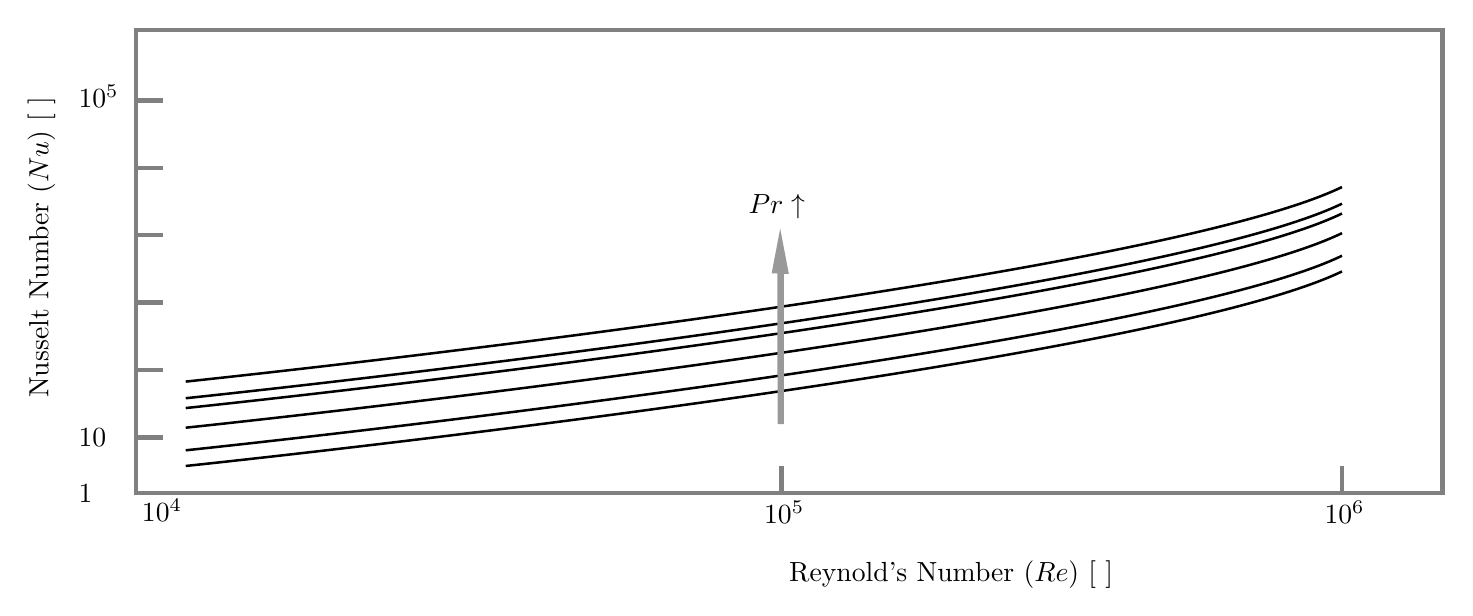
\begin{tikzpicture}[y=0.80pt, x=0.8pt,yscale=-1, inner sep=0pt, outer sep=0pt]
\begin{scope}[shift={(0,-782.35975)}]
  \path[draw=c808080,miter limit=4.00,line width=1.600pt,rounded corners=0.0000cm]
    (70.4594,794.8260) rectangle (660.5406,1003.8935);
  \path[draw=c808080,line join=miter,line cap=butt,miter limit=4.00,line
    width=1.600pt] (70.4594,826.6674) -- (82.4417,826.6674);
  \path[draw=c808080,line join=miter,line cap=butt,miter limit=4.00,line
    width=1.600pt] (70.4594,978.8864) -- (82.4417,978.8864);
  \path[draw=c808080,line join=miter,line cap=butt,miter limit=4.00,line
    width=1.600pt] (362.0178,1003.8935) -- (362.0178,991.9113);
  \path[draw=c808080,line join=miter,line cap=butt,miter limit=4.00,line
    width=1.600pt] (615.1302,1003.8935) -- (615.1302,991.9113);
  \path[fill=c999999] (44.4142,830.09515) node[above right] (text3839) {$10^{5}$};
  \path[fill=c999999] (44.4142,1008.4214) node[above right] (text3843) {$1$};
  \path[fill=c999999] (73.039719,1017.0943) node[above right] (text3847-2-5)
    {$10^{4}$};
  \path[fill=c999999] (354.08807,1017.9819) node[above right] (text3847-2-5-1)
    {$10^{5}$};
  \path[fill=c999999] (607.2005,1017.9819) node[above right] (text3847-2-5-2)
    {$10^{6}$};
  \path[fill=c999999] (365.41504,1047.0343) node[above right] (text3932)
    {Reynold's Number ($Re$) [ ]};
  \path[cm={{0.0,-1.0,1.0,0.0,(0.0,0.0)}},fill=c999999] (-961.04724,21.434233)
    node[above right] (text3932-1) {\rotatebox{90}{Nusselt Number ($Nu$) [ ]}};
  \path[draw=black,line join=miter,line cap=butt,line width=0.910pt]
    (615.0888,896.8450) .. controls (526.7055,939.4485) and (92.8241,984.7148) ..
    (92.8241,984.7148);
  \path[draw=black,line join=miter,line cap=butt,line width=0.910pt]
    (615.0888,886.6379) .. controls (526.7055,929.2414) and (92.8241,974.5077) ..
    (92.8241,974.5077);
  \path[draw=black,line join=miter,line cap=butt,line width=0.910pt]
    (615.0888,877.7621) .. controls (526.7055,920.3657) and (92.8241,965.6319) ..
    (92.8241,965.6319);
  \path[draw=black,line join=miter,line cap=butt,line width=0.910pt]
    (615.0888,865.8095) .. controls (526.7055,908.4130) and (92.8241,953.6793) ..
    (92.8241,953.6793);
  \path[draw=black,line join=miter,line cap=butt,line width=0.910pt]
    (615.0888,873.3243) .. controls (526.7055,915.9278) and (92.8241,961.1941) ..
    (92.8241,961.1941);
  \path[draw=black,line join=miter,line cap=butt,line width=0.910pt]
    (615.0888,903.9278) .. controls (526.7055,946.5313) and (92.8241,991.7976) ..
    (92.8241,991.7976);
  \path[fill=black] (347.04138,880.17041) node[above right] (text4030) {$Pr
    \uparrow$};
  \path[draw=c808080,line join=miter,line cap=butt,miter limit=4.00,line
    width=1.600pt] (70.4594,948.4426) -- (82.4417,948.4426);
  \path[draw=c808080,line join=miter,line cap=butt,miter limit=4.00,line
    width=1.600pt] (70.4594,917.9988) -- (82.4417,917.9988);
  \path[draw=c808080,line join=miter,line cap=butt,miter limit=4.00,line
    width=1.600pt] (70.4594,887.5550) -- (82.4417,887.5550);
  \path[draw=c808080,line join=miter,line cap=butt,miter limit=4.00,line
    width=1.600pt] (70.4594,857.1112) -- (82.4417,857.1112);
  \path[fill=c999999] (44.4142,982.95862) node[above right] (text3843-4) {$10$};
  \path[fill=c999999] (360.1441,972.9219) -- (362.9450,972.9219) --
    (362.9450,905.0225) -- (365.2367,905.0225) -- (361.3323,884.6083) --
    (357.4704,904.8006) -- (360.0592,904.8006) -- cycle;
\end{scope}

\end{tikzpicture}
